
\documentclass[../main.tex]{subfiles}
\graphicspath{{\subfix{../images/}}}
\begin{document}
\textbf{....}
        \begin{figure}[bh]
        \centering
        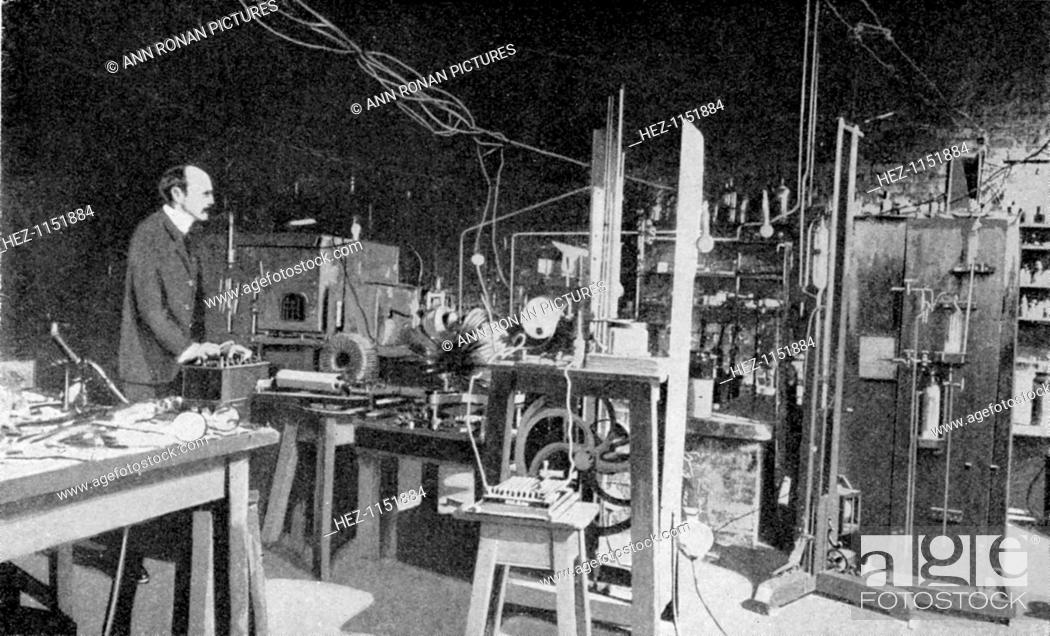
\includegraphics[width=3cm]{01.JJ-THOMSON-LAB}
        \label{fig:img1}
        \caption{JJ Thomson}
    \end{figure}
    
\begin{enumerate}[I. ]
    \item \href{https://www.webassign.net/question_assets/unccolphyseml1/lab_4/manual.html}{Determination of e/m for the Electron}
    \item \href{https://physicsx.erau.edu/HelmholtzCoils/Lab_MP_1.pdf}{e/m ratio of the electron}
    \item \href{https://virtuelle-experimente.de/en/b-feld/e-m-bestimmung/edurchm.php}{Use the experiment to measure the ratio of the electrons charge to it's mass.}{}
    \item \href{https://www.physik.uzh.ch/~matthias/espace-assistant/manuals/en/anleitung_etom_e.pdf}{4. Electron Charge-to-Mass Ratio e/m - UZH - Physik-Institut}
    \item \href{https://demoweb.physics.ucla.edu/6b-lab-manual}{UCLA Physics \& Astronomy}
     \item \href{https://www.famousscientists.org/j-j-thomson/}{J. J. Thomson. Famous Scientists -The Art of Genius-}
     \item \href{https://virtuelle-experimente.de/en/index.php}{Electron Motion in Electric and Magnetic Fields}
\end{enumerate}

\begin{enumerate}[1. ]
    \item \href{https://www.physicsread.com/latex-vector-bold/}{LATEX Physicsread}
    \item \href{https://physicsanduniverse.com/latex-symbols-and-using-them-to-write-equations/}{LaTeX Symbols and using them to write Equations}
    \item \href{https://texdoc.org/serve/siunitx/0}{siunitx – A comprehensive (SI) units package}
    \item \href{http://math.univ-lyon1.fr/irem/IMG/pdf/LatexPourLeProfDeMaths.pdf}{LATEX... pour le prof de maths }
\end{enumerate}
\end{document}


